\documentclass[]{article}
\usepackage{lmodern}
\usepackage{amssymb,amsmath}
\usepackage{ifxetex,ifluatex}
\usepackage{fixltx2e} % provides \textsubscript
\ifnum 0\ifxetex 1\fi\ifluatex 1\fi=0 % if pdftex
  \usepackage[T1]{fontenc}
  \usepackage[utf8]{inputenc}
\else % if luatex or xelatex
  \ifxetex
    \usepackage{mathspec}
  \else
    \usepackage{fontspec}
  \fi
  \defaultfontfeatures{Ligatures=TeX,Scale=MatchLowercase}
\fi
% use upquote if available, for straight quotes in verbatim environments
\IfFileExists{upquote.sty}{\usepackage{upquote}}{}
% use microtype if available
\IfFileExists{microtype.sty}{%
\usepackage{microtype}
\UseMicrotypeSet[protrusion]{basicmath} % disable protrusion for tt fonts
}{}
\usepackage[margin=1in]{geometry}
\usepackage{hyperref}
\hypersetup{unicode=true,
            pdftitle={Network analysis tutorial},
            pdfauthor={Jiaxin Deng},
            pdfborder={0 0 0},
            breaklinks=true}
\urlstyle{same}  % don't use monospace font for urls
\usepackage{color}
\usepackage{fancyvrb}
\newcommand{\VerbBar}{|}
\newcommand{\VERB}{\Verb[commandchars=\\\{\}]}
\DefineVerbatimEnvironment{Highlighting}{Verbatim}{commandchars=\\\{\}}
% Add ',fontsize=\small' for more characters per line
\usepackage{framed}
\definecolor{shadecolor}{RGB}{248,248,248}
\newenvironment{Shaded}{\begin{snugshade}}{\end{snugshade}}
\newcommand{\KeywordTok}[1]{\textcolor[rgb]{0.13,0.29,0.53}{\textbf{#1}}}
\newcommand{\DataTypeTok}[1]{\textcolor[rgb]{0.13,0.29,0.53}{#1}}
\newcommand{\DecValTok}[1]{\textcolor[rgb]{0.00,0.00,0.81}{#1}}
\newcommand{\BaseNTok}[1]{\textcolor[rgb]{0.00,0.00,0.81}{#1}}
\newcommand{\FloatTok}[1]{\textcolor[rgb]{0.00,0.00,0.81}{#1}}
\newcommand{\ConstantTok}[1]{\textcolor[rgb]{0.00,0.00,0.00}{#1}}
\newcommand{\CharTok}[1]{\textcolor[rgb]{0.31,0.60,0.02}{#1}}
\newcommand{\SpecialCharTok}[1]{\textcolor[rgb]{0.00,0.00,0.00}{#1}}
\newcommand{\StringTok}[1]{\textcolor[rgb]{0.31,0.60,0.02}{#1}}
\newcommand{\VerbatimStringTok}[1]{\textcolor[rgb]{0.31,0.60,0.02}{#1}}
\newcommand{\SpecialStringTok}[1]{\textcolor[rgb]{0.31,0.60,0.02}{#1}}
\newcommand{\ImportTok}[1]{#1}
\newcommand{\CommentTok}[1]{\textcolor[rgb]{0.56,0.35,0.01}{\textit{#1}}}
\newcommand{\DocumentationTok}[1]{\textcolor[rgb]{0.56,0.35,0.01}{\textbf{\textit{#1}}}}
\newcommand{\AnnotationTok}[1]{\textcolor[rgb]{0.56,0.35,0.01}{\textbf{\textit{#1}}}}
\newcommand{\CommentVarTok}[1]{\textcolor[rgb]{0.56,0.35,0.01}{\textbf{\textit{#1}}}}
\newcommand{\OtherTok}[1]{\textcolor[rgb]{0.56,0.35,0.01}{#1}}
\newcommand{\FunctionTok}[1]{\textcolor[rgb]{0.00,0.00,0.00}{#1}}
\newcommand{\VariableTok}[1]{\textcolor[rgb]{0.00,0.00,0.00}{#1}}
\newcommand{\ControlFlowTok}[1]{\textcolor[rgb]{0.13,0.29,0.53}{\textbf{#1}}}
\newcommand{\OperatorTok}[1]{\textcolor[rgb]{0.81,0.36,0.00}{\textbf{#1}}}
\newcommand{\BuiltInTok}[1]{#1}
\newcommand{\ExtensionTok}[1]{#1}
\newcommand{\PreprocessorTok}[1]{\textcolor[rgb]{0.56,0.35,0.01}{\textit{#1}}}
\newcommand{\AttributeTok}[1]{\textcolor[rgb]{0.77,0.63,0.00}{#1}}
\newcommand{\RegionMarkerTok}[1]{#1}
\newcommand{\InformationTok}[1]{\textcolor[rgb]{0.56,0.35,0.01}{\textbf{\textit{#1}}}}
\newcommand{\WarningTok}[1]{\textcolor[rgb]{0.56,0.35,0.01}{\textbf{\textit{#1}}}}
\newcommand{\AlertTok}[1]{\textcolor[rgb]{0.94,0.16,0.16}{#1}}
\newcommand{\ErrorTok}[1]{\textcolor[rgb]{0.64,0.00,0.00}{\textbf{#1}}}
\newcommand{\NormalTok}[1]{#1}
\usepackage{graphicx,grffile}
\makeatletter
\def\maxwidth{\ifdim\Gin@nat@width>\linewidth\linewidth\else\Gin@nat@width\fi}
\def\maxheight{\ifdim\Gin@nat@height>\textheight\textheight\else\Gin@nat@height\fi}
\makeatother
% Scale images if necessary, so that they will not overflow the page
% margins by default, and it is still possible to overwrite the defaults
% using explicit options in \includegraphics[width, height, ...]{}
\setkeys{Gin}{width=\maxwidth,height=\maxheight,keepaspectratio}
\IfFileExists{parskip.sty}{%
\usepackage{parskip}
}{% else
\setlength{\parindent}{0pt}
\setlength{\parskip}{6pt plus 2pt minus 1pt}
}
\setlength{\emergencystretch}{3em}  % prevent overfull lines
\providecommand{\tightlist}{%
  \setlength{\itemsep}{0pt}\setlength{\parskip}{0pt}}
\setcounter{secnumdepth}{0}
% Redefines (sub)paragraphs to behave more like sections
\ifx\paragraph\undefined\else
\let\oldparagraph\paragraph
\renewcommand{\paragraph}[1]{\oldparagraph{#1}\mbox{}}
\fi
\ifx\subparagraph\undefined\else
\let\oldsubparagraph\subparagraph
\renewcommand{\subparagraph}[1]{\oldsubparagraph{#1}\mbox{}}
\fi

%%% Use protect on footnotes to avoid problems with footnotes in titles
\let\rmarkdownfootnote\footnote%
\def\footnote{\protect\rmarkdownfootnote}

%%% Change title format to be more compact
\usepackage{titling}

% Create subtitle command for use in maketitle
\providecommand{\subtitle}[1]{
  \posttitle{
    \begin{center}\large#1\end{center}
    }
}

\setlength{\droptitle}{-2em}

  \title{Network analysis tutorial}
    \pretitle{\vspace{\droptitle}\centering\huge}
  \posttitle{\par}
    \author{Jiaxin Deng}
    \preauthor{\centering\large\emph}
  \postauthor{\par}
      \predate{\centering\large\emph}
  \postdate{\par}
    \date{2019/5/20}


\begin{document}
\maketitle

\section{Brief introduction to network
analysis}\label{brief-introduction-to-network-analysis}

A network is a set of nodes connected by a set of edges.

Several packages are used in the network analysis, including
\texttt{network}, \texttt{statnet}, \texttt{igraph} and \texttt{qgraph}.

\texttt{qgraph} was developed in the context of psychometrics approach
by Dr.~Sacha Epskamp and colleagues in 2012. For more details, please
click this following link for the paper published in \emph{Journal of
Statistical Softare}:

\url{https://www.jstatsoft.org/article/view/v048i04}

This package can create graphs to visualize the statistics in different
layout modes based on different correlation matrices, such as polychoric
correlation, partial correlation.

\section{Example code}\label{example-code}

Here is some example code to show how to conduct a network analysis.

\subsection{Estimating networks}\label{estimating-networks}

\subsubsection{How to make a graph}\label{how-to-make-a-graph}

Here is the following steps to make a gragh using \texttt{qgraph}.

Take \texttt{big5} data as an example. This is a dataset of the Big five
personality traits assessed on 500 psychology students.

Firstly, \texttt{qgraph} package should be activated using
\texttt{library()}

\begin{Shaded}
\begin{Highlighting}[]
\KeywordTok{library}\NormalTok{(qgraph)}
\end{Highlighting}
\end{Shaded}

And then, data need to be imported in the current R project.

\begin{Shaded}
\begin{Highlighting}[]
\KeywordTok{data}\NormalTok{(big5)}
\end{Highlighting}
\end{Shaded}

To creat the graph is basically to use \texttt{qgraph()}, such as:

\begin{Shaded}
\begin{Highlighting}[]
\NormalTok{qgraph<-}\KeywordTok{qgraph}\NormalTok{(}\KeywordTok{cor}\NormalTok{(big5))}
\end{Highlighting}
\end{Shaded}

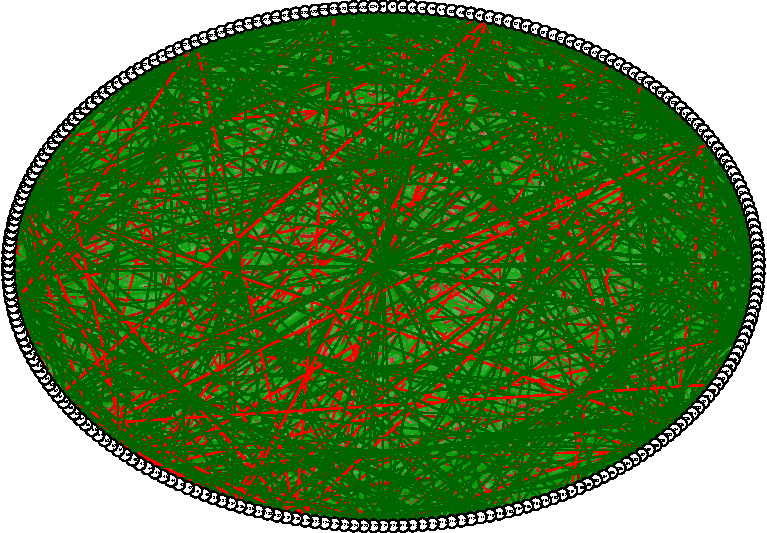
\includegraphics{tutorial_files/figure-latex/cor big5-1.pdf}

But it should be noted that the input in the \texttt{qgraph()} can be a
weight matrix or an edgelist.

Thus, if you want to creat the association network,
\texttt{cor()}/\texttt{cor\_auto()} can be used to creat the matrix
first.

Also, you can use \texttt{groups} to indicate which nodes belong
together, such as:

\begin{Shaded}
\begin{Highlighting}[]
\KeywordTok{data}\NormalTok{(}\StringTok{"big5groups"}\NormalTok{)}
\KeywordTok{qgraph}\NormalTok{(}\KeywordTok{cor}\NormalTok{(big5), }\DataTypeTok{groups=}\NormalTok{big5groups)}
\end{Highlighting}
\end{Shaded}

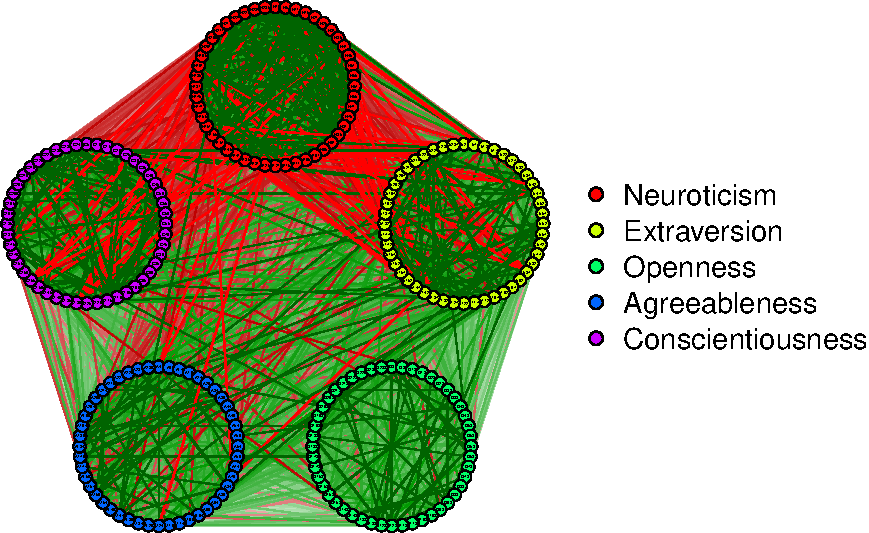
\includegraphics{tutorial_files/figure-latex/groups big5-1.pdf}

Besides, you can use some additional arguments to customize your
representing graph.

you can use \texttt{layout} to change the representation, such as:

\begin{Shaded}
\begin{Highlighting}[]
\KeywordTok{qgraph}\NormalTok{(}\KeywordTok{cor}\NormalTok{(big5), }\DataTypeTok{groups=}\NormalTok{big5groups,}\DataTypeTok{layout=} \StringTok{"spring"}\NormalTok{)}
\end{Highlighting}
\end{Shaded}

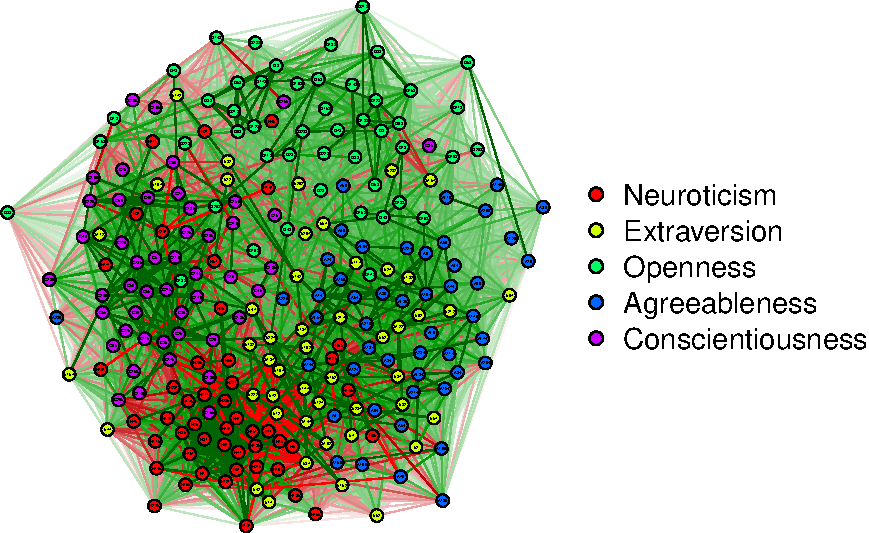
\includegraphics{tutorial_files/figure-latex/layout big5-1.pdf}

\begin{Shaded}
\begin{Highlighting}[]
\KeywordTok{qgraph}\NormalTok{(}\KeywordTok{cor}\NormalTok{(big5), }\DataTypeTok{groups=}\NormalTok{big5groups,}\DataTypeTok{layout=} \StringTok{"circle"}\NormalTok{)}
\end{Highlighting}
\end{Shaded}

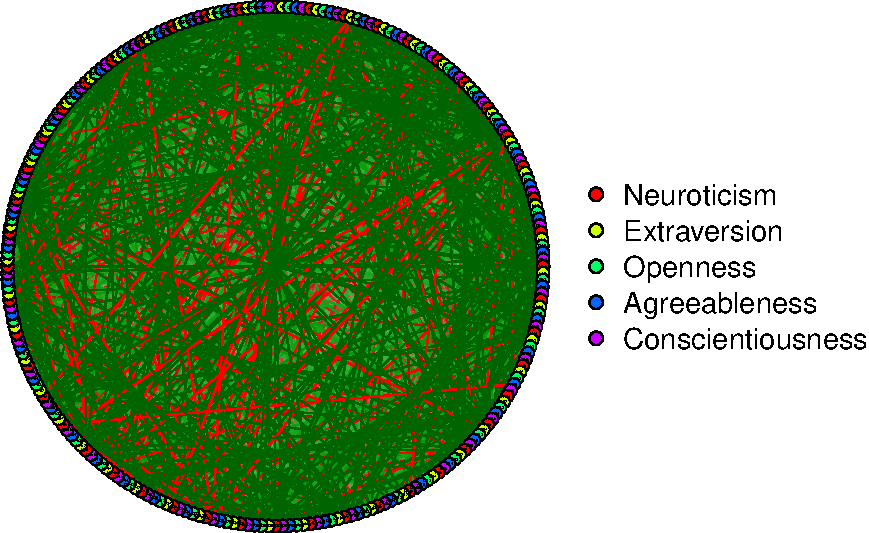
\includegraphics{tutorial_files/figure-latex/layout2 big5-1.pdf}

Moreover, you can use \texttt{palette} and \texttt{theme} to change the
colour of nodes.

Notes: the palette used for colouring nodes when using \texttt{groups}
argument.

For example:

\begin{Shaded}
\begin{Highlighting}[]
\KeywordTok{qgraph}\NormalTok{(}\KeywordTok{cor}\NormalTok{(big5), }\DataTypeTok{groups=}\NormalTok{big5groups,}\DataTypeTok{palette=}\StringTok{"colorblind"}\NormalTok{)}
\end{Highlighting}
\end{Shaded}

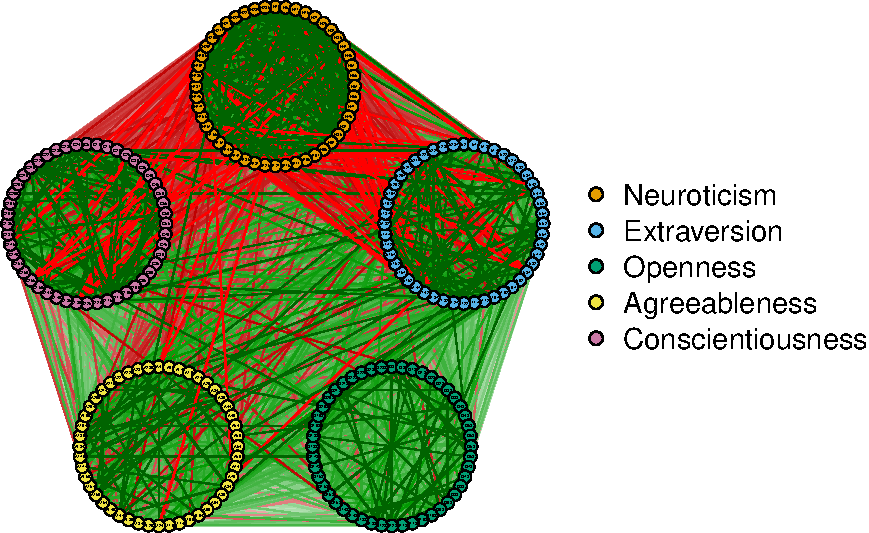
\includegraphics{tutorial_files/figure-latex/pa big5-1.pdf}

More specifically, there are several optional graphical arguments to
change the graph representation, such as \texttt{minizum} (to omit
correlations not interested in), \texttt{borders}(to omit borders around
the nodes), \texttt{vsize}(to change the size of nodes) and
\texttt{legend}(to control the legend placed on the right side).

For example:

\begin{Shaded}
\begin{Highlighting}[]
\KeywordTok{qgraph}\NormalTok{(}\KeywordTok{cor}\NormalTok{(big5), }\DataTypeTok{groups=}\NormalTok{big5groups,}\DataTypeTok{layout=}\StringTok{"spring"}\NormalTok{,}\DataTypeTok{minimum=}\FloatTok{0.35}\NormalTok{,}\DataTypeTok{vsize=}\DecValTok{3}\NormalTok{,}\DataTypeTok{legend=}\OtherTok{TRUE}\NormalTok{,}\DataTypeTok{borders=}\OtherTok{FALSE}\NormalTok{)}
\end{Highlighting}
\end{Shaded}

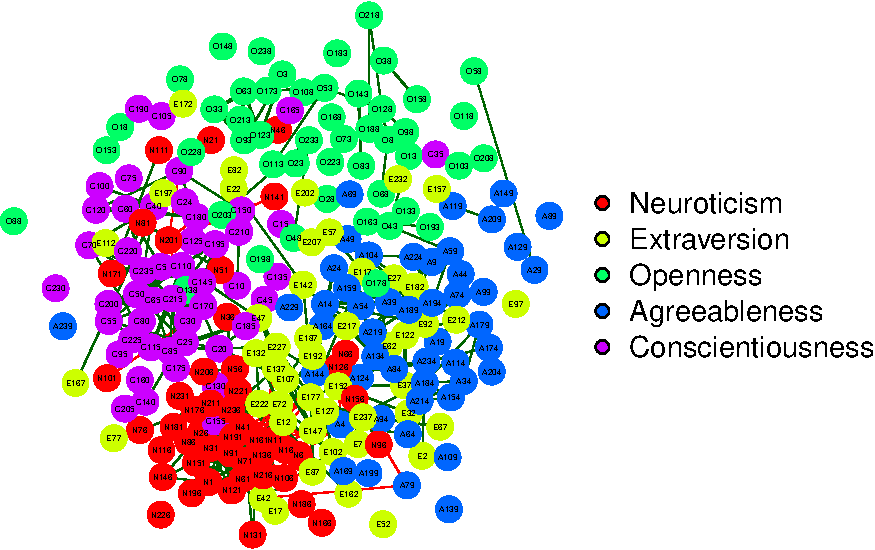
\includegraphics{tutorial_files/figure-latex/additional big5-1.pdf}

In addition, there are some options for correlation or covariance
matrices to make the graph. You can use \texttt{graph} to change the
type of graph.

For example, if you want to plot a partial correlation network, you can
use \texttt{graph="pcor} to make it.

\begin{Shaded}
\begin{Highlighting}[]
\KeywordTok{qgraph}\NormalTok{(}\KeywordTok{cor}\NormalTok{(big5), }\DataTypeTok{groups=}\NormalTok{big5groups,}\DataTypeTok{layout=}\StringTok{"spring"}\NormalTok{,}\DataTypeTok{minimum=}\FloatTok{0.35}\NormalTok{,}\DataTypeTok{vsize=}\DecValTok{3}\NormalTok{,}\DataTypeTok{legend=}\OtherTok{TRUE}\NormalTok{,}\DataTypeTok{borders=}\OtherTok{FALSE}\NormalTok{,}\DataTypeTok{graph=}\StringTok{"pcor"}\NormalTok{)}
\end{Highlighting}
\end{Shaded}

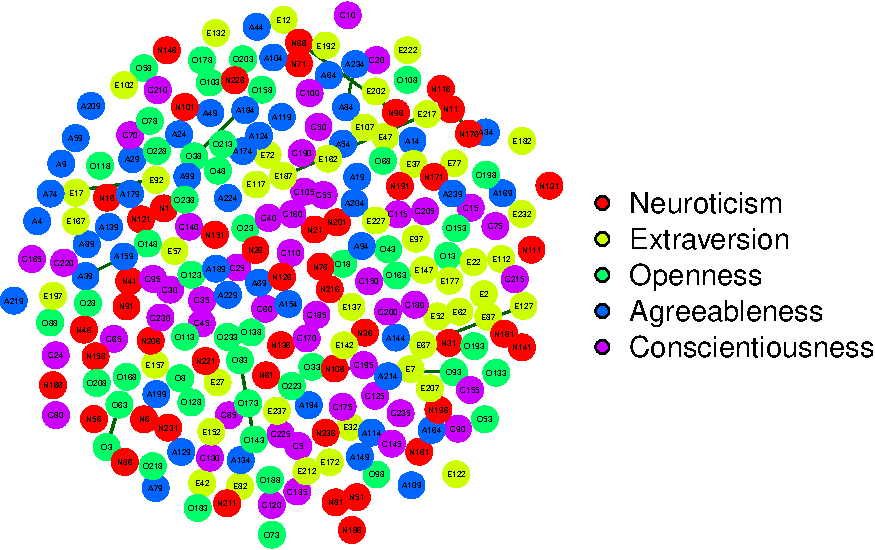
\includegraphics{tutorial_files/figure-latex/graph big5-1.pdf}

Finally, if you decide the representation of the graph, you can choose
to use \texttt{filetype}(pdf/jpg/tex etc.) to save your graph.

\subsubsection{How to calculate the centrality
indices}\label{how-to-calculate-the-centrality-indices}

After estimating the graph, you can calculate the centrality indices
using \texttt{centralityPlot} to quantify the structural importance of
each node in the network.

Then, you will get this figure.

\begin{verbatim}
## Note: z-scores are shown on x-axis rather than raw centrality indices.
\end{verbatim}

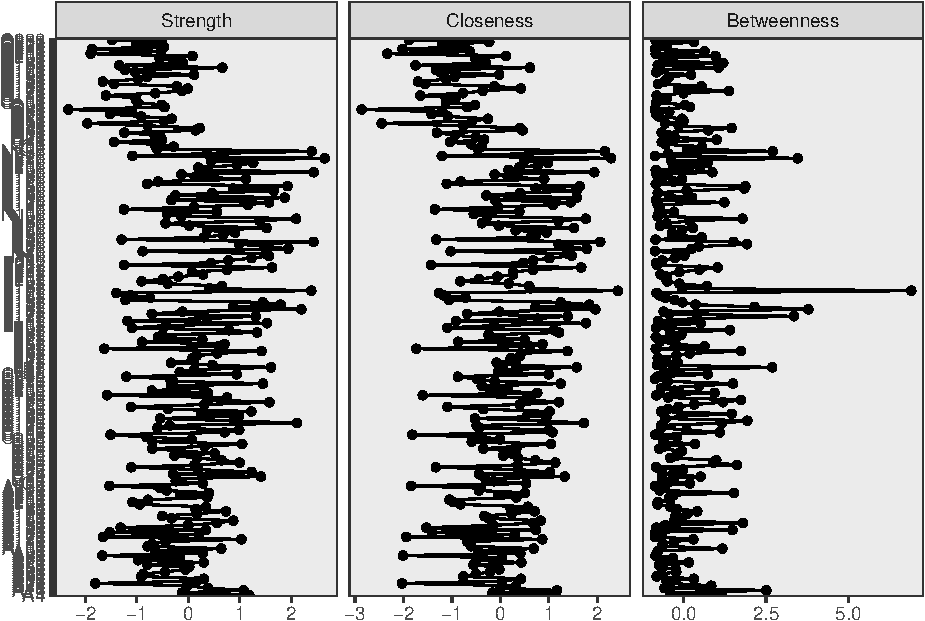
\includegraphics{tutorial_files/figure-latex/centrality big5-1.pdf}

\subsection{Estimating the accuracy of
networks}\label{estimating-the-accuracy-of-networks}

Like many psychometrics analysis, the accuracy of psychological network
is also limited to sample size. The limited sample size might restrict
the accuracy of the parameters and the interpretation of the network.
Thus, it's necessary and crucial to assess the accuracy of the network
parameters and measures.

In order to estimate the accuracy of the networks estimation, three
steps to evaluate the stability of the network routinely were conducted
using \texttt{bootnet} package
\href{https://link.springer.com/article/10.3758/s13428-017-0862-1}{(Epskamp,
Borsboom \& Fried, 2018)}

In addition to use \texttt{qgraph} to create the graph, you can also use
\texttt{estimateNetwork} to estimate the network structure as well.

To get the data:

\begin{Shaded}
\begin{Highlighting}[]
\KeywordTok{library}\NormalTok{(psych)}
\KeywordTok{data}\NormalTok{(}\StringTok{"bfi"}\NormalTok{)}
\NormalTok{bfisub<-bfi[}\DecValTok{1}\OperatorTok{:}\DecValTok{100}\NormalTok{,}\DecValTok{1}\OperatorTok{:}\DecValTok{25}\NormalTok{]}
\end{Highlighting}
\end{Shaded}

\begin{Shaded}
\begin{Highlighting}[]
\KeywordTok{library}\NormalTok{(bootnet)}
\end{Highlighting}
\end{Shaded}

\begin{verbatim}
## Loading required package: ggplot2
\end{verbatim}

\begin{verbatim}
## 
## Attaching package: 'ggplot2'
\end{verbatim}

\begin{verbatim}
## The following objects are masked from 'package:psych':
## 
##     %+%, alpha
\end{verbatim}

\begin{verbatim}
## This is bootnet 1.2
\end{verbatim}

\begin{verbatim}
## For questions and issues, please see github.com/SachaEpskamp/bootnet.
\end{verbatim}

\begin{Shaded}
\begin{Highlighting}[]
\NormalTok{Network <-}\StringTok{ }\KeywordTok{estimateNetwork}\NormalTok{(bfisub, }\DataTypeTok{default =} \StringTok{"cor"}\NormalTok{)}
\end{Highlighting}
\end{Shaded}

\begin{verbatim}
## Estimating Network. Using package::function:
##   - qgraph::cor_auto for correlation computation
##     - using lavaan::lavCor
##   - psych::corr.p for significance thresholding
\end{verbatim}

\begin{verbatim}
## Variables detected as ordinal: A1; A2; A3; A4; A5; C1; C2; C3; C4; C5; E1; E2; E3; E4; E5; N1; N2; N3; N4; N5; O1; O2; O3; O4; O5
\end{verbatim}

\begin{Shaded}
\begin{Highlighting}[]
\KeywordTok{plot}\NormalTok{(Network, }\DataTypeTok{layout =} \StringTok{'spring'}\NormalTok{)}
\end{Highlighting}
\end{Shaded}

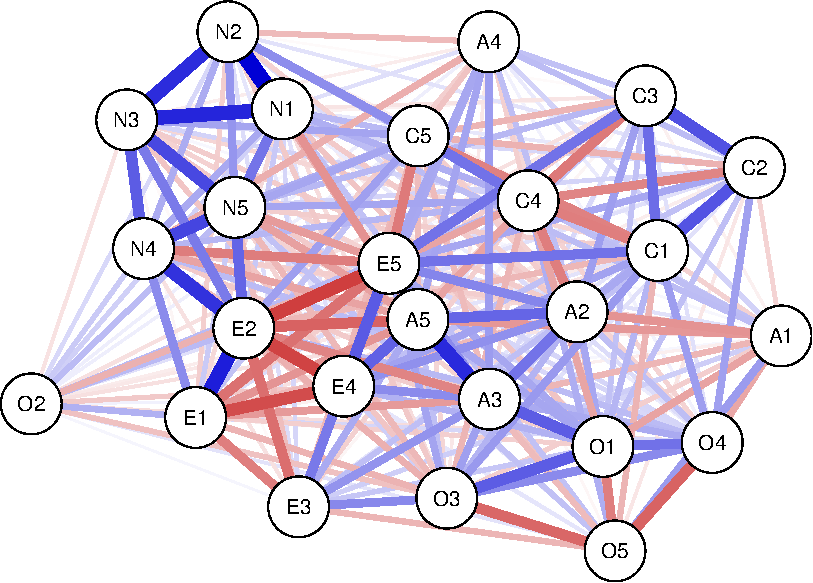
\includegraphics{tutorial_files/figure-latex/network-1.pdf}

Here is three steps to conduct the accuracy estimation.

Firstly, the accuracy of edge-weights can be estimated by drawing
bootstrapped CIs.

\begin{Shaded}
\begin{Highlighting}[]
\NormalTok{Results1 <-}\StringTok{ }\KeywordTok{bootnet}\NormalTok{(Network, }\DataTypeTok{nBoots =} \DecValTok{1000}\NormalTok{, }\DataTypeTok{nCores =} \DecValTok{8}\NormalTok{)}
\end{Highlighting}
\end{Shaded}

\begin{verbatim}
## Note: bootnet will store only the following statistics:  edge, strength, outStrength, inStrength
\end{verbatim}

\begin{verbatim}
## Estimating sample network...
\end{verbatim}

\begin{verbatim}
## Estimating Network. Using package::function:
##   - qgraph::cor_auto for correlation computation
##     - using lavaan::lavCor
##   - psych::corr.p for significance thresholding
\end{verbatim}

\begin{verbatim}
## Variables detected as ordinal: A1; A2; A3; A4; A5; C1; C2; C3; C4; C5; E1; E2; E3; E4; E5; N1; N2; N3; N4; N5; O1; O2; O3; O4; O5
\end{verbatim}

\begin{verbatim}
## Bootstrapping...
\end{verbatim}

\begin{verbatim}
## Computing statistics...
\end{verbatim}

\begin{Shaded}
\begin{Highlighting}[]
\KeywordTok{plot}\NormalTok{(Results1, }\DataTypeTok{labels =} \OtherTok{FALSE}\NormalTok{, }\DataTypeTok{order =} \StringTok{"sample"}\NormalTok{)}
\end{Highlighting}
\end{Shaded}

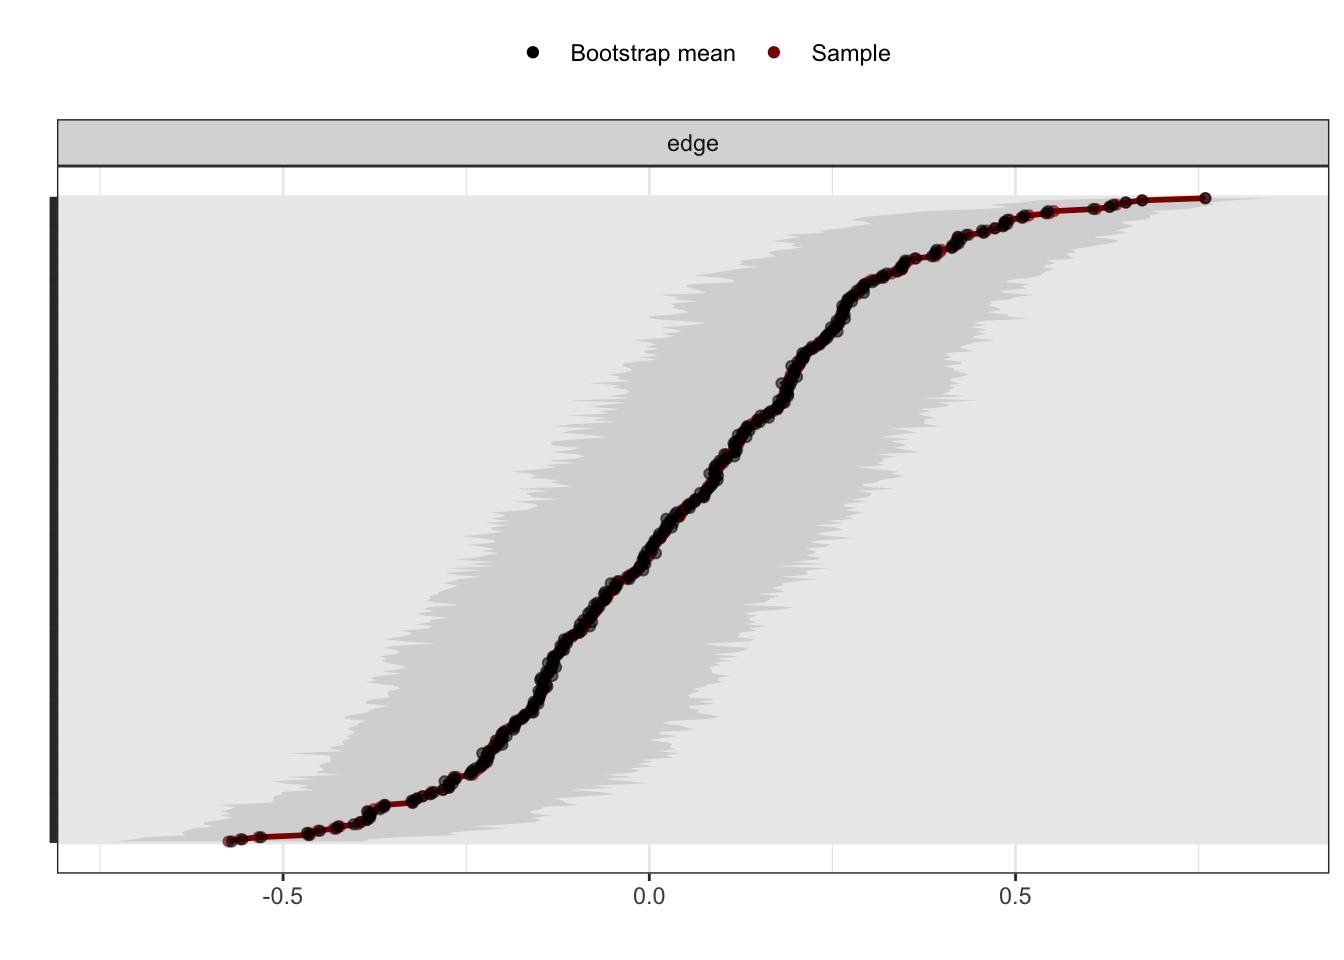
\includegraphics{tutorial_files/figure-latex/edge-weight-1.pdf}

Secondly, the stability of centrality indices can be investigated after
observation only portions of the data.

\begin{Shaded}
\begin{Highlighting}[]
\NormalTok{Results2 <-}\StringTok{ }\KeywordTok{bootnet}\NormalTok{(Network, }\DataTypeTok{nBoots =} \DecValTok{1000}\NormalTok{, }\DataTypeTok{nCores =} \DecValTok{8}\NormalTok{, }\DataTypeTok{type =} \StringTok{"case"}\NormalTok{)}
\end{Highlighting}
\end{Shaded}

\begin{verbatim}
## Note: bootnet will store only the following statistics:  edge, strength, outStrength, inStrength
\end{verbatim}

\begin{verbatim}
## Estimating sample network...
\end{verbatim}

\begin{verbatim}
## Estimating Network. Using package::function:
##   - qgraph::cor_auto for correlation computation
##     - using lavaan::lavCor
##   - psych::corr.p for significance thresholding
\end{verbatim}

\begin{verbatim}
## Variables detected as ordinal: A1; A2; A3; A4; A5; C1; C2; C3; C4; C5; E1; E2; E3; E4; E5; N1; N2; N3; N4; N5; O1; O2; O3; O4; O5
\end{verbatim}

\begin{verbatim}
## Bootstrapping...
\end{verbatim}

\begin{verbatim}
## Computing statistics...
\end{verbatim}

\begin{Shaded}
\begin{Highlighting}[]
\KeywordTok{plot}\NormalTok{(Results2)}
\end{Highlighting}
\end{Shaded}

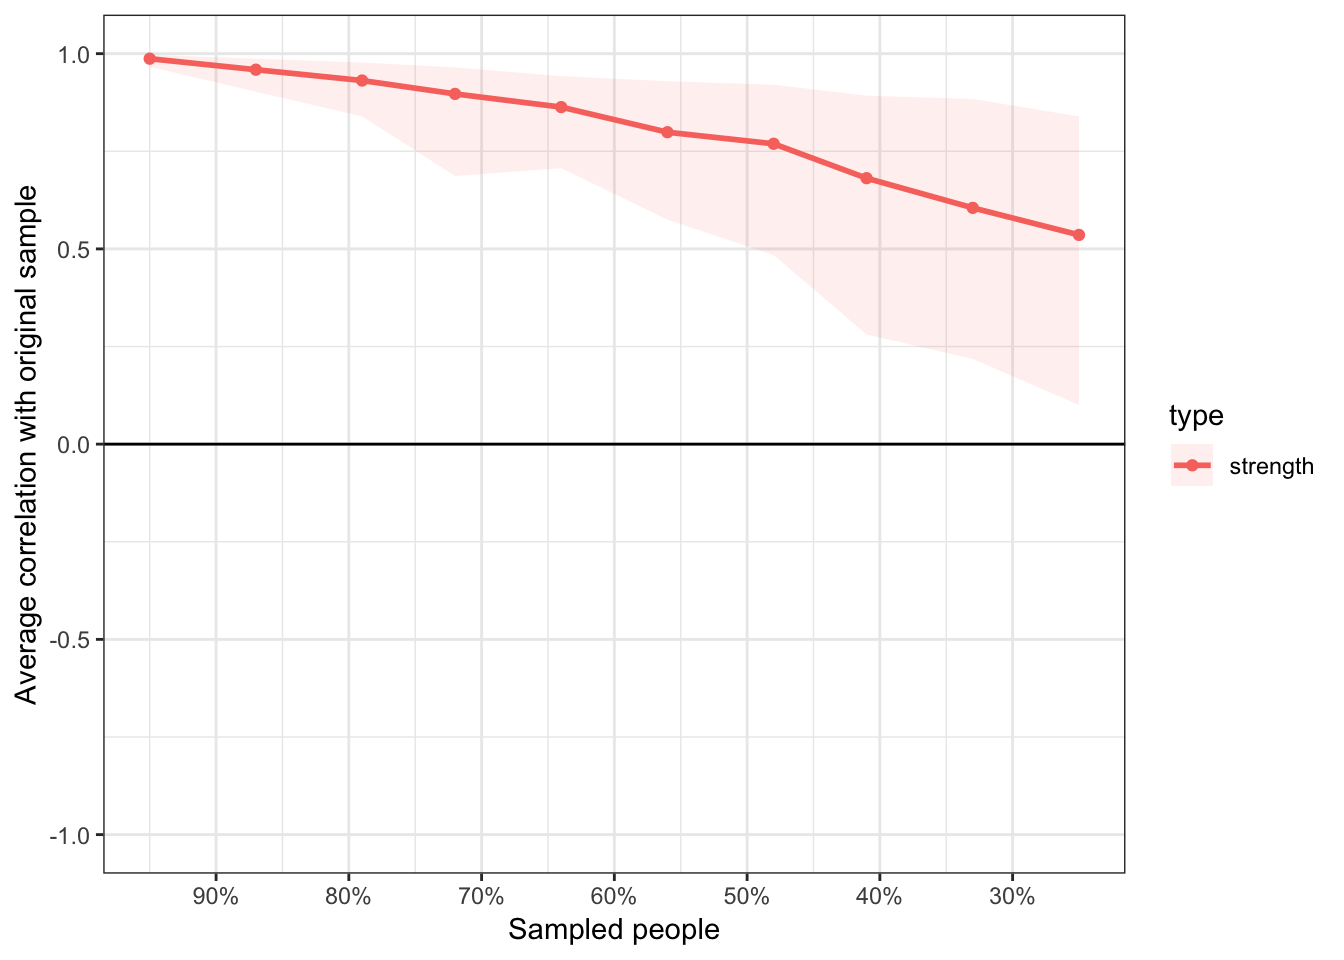
\includegraphics{tutorial_files/figure-latex/centrality-1.pdf}

Lastly, the bootstrapped differences between edge-weights and centrality
indices to test whether these differ significantly from each other can
be carried out.

\begin{Shaded}
\begin{Highlighting}[]
\KeywordTok{plot}\NormalTok{(Results1, }\StringTok{"edge"}\NormalTok{, }\DataTypeTok{plot =} \StringTok{"difference"}\NormalTok{,}\DataTypeTok{onlyNonZero =} \OtherTok{TRUE}\NormalTok{, }\DataTypeTok{order =} \StringTok{"sample"}\NormalTok{)}
\end{Highlighting}
\end{Shaded}

\begin{verbatim}
## Expected significance level given number of bootstrap samples is approximately: 0.05
\end{verbatim}

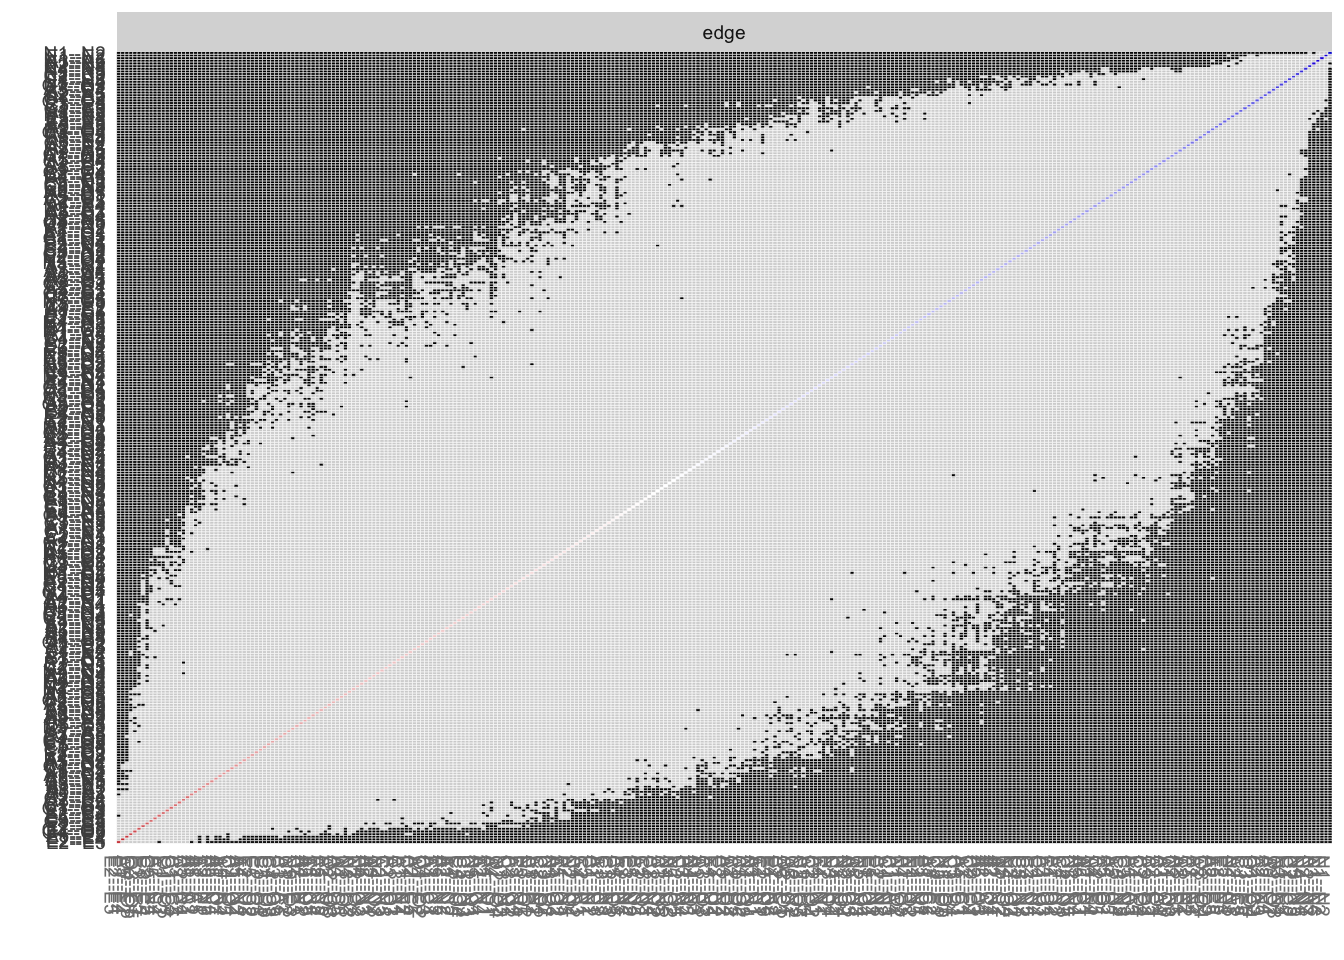
\includegraphics{tutorial_files/figure-latex/diffedge-1.pdf}

\begin{Shaded}
\begin{Highlighting}[]
\KeywordTok{plot}\NormalTok{(Results1, }\StringTok{"strength"}\NormalTok{, }\DataTypeTok{plot =} \StringTok{"difference"}\NormalTok{)}
\end{Highlighting}
\end{Shaded}

\begin{verbatim}
## Expected significance level given number of bootstrap samples is approximately: 0.05
\end{verbatim}

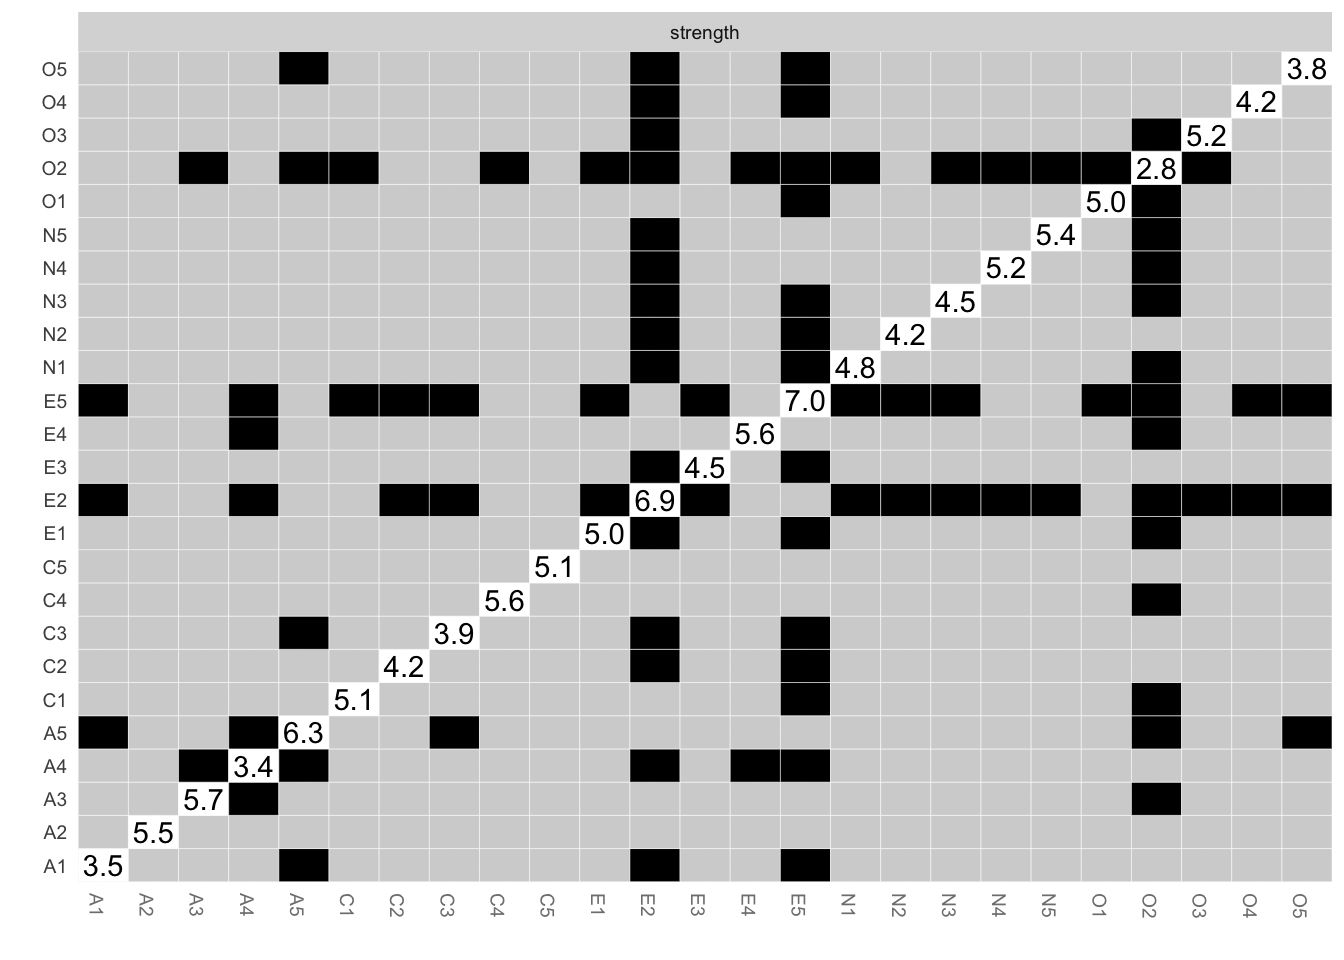
\includegraphics{tutorial_files/figure-latex/diffstrength-1.pdf}


\end{document}
